\documentclass[11pt,a4paper]{article}
\usepackage[T1]{fontenc}
\usepackage[margin=2.3cm]{geometry}
\usepackage{amsmath,amssymb}
\usepackage{graphicx}
\usepackage[dvipsnames]{xcolor}
\usepackage{enumitem}
\usepackage[colorlinks=true,linkcolor=blue,urlcolor=blue]{hyperref}
\setlength{\parskip}{0.6em}
\setlength{\parindent}{0pt}
\begin{document}

\begin{center}{\LARGE\bfseries openledcontrol}\\[0.4em]{\large Build a light-activated LED controller, from an LDR to a transistor switch, in three sessions.}\\[0.2em]\small PAN IIT OSS explainer \textbullet{} secondary school to diploma / undergraduate (levels 3-5)\end{center}

\section*{Why this exists}
A light that switches itself on is a small machine made of four jobs: sense the light, decide that it is dark, switch a larger current, and light a lamp. This explainer follows each job with a formula and a simulation, using only a voltage divider, a transistor and a few gates, so you can build it yourself.

\section*{The end goal}
Build a light-activated LED controller with a sensor and transistor switch. The end goal is a light-activated LED controller with a sensor and transistor switch, as found in street lights, garden lights and night lights. The same ideas of divider, threshold, hysteresis and logic appear in thermostats, alarms and many other low-voltage control circuits.

\section*{How the three sessions build up}
\begin{enumerate}[nosep]
\item \textbf{Session 1: A sensor, a decision and a switch} (Level 1, conceptual interactive model, 60 min).
\item \textbf{Session 2: The divider, the LED resistor and the transistor} (Level 2, mathematical engineering model, 75 min).
\item \textbf{Session 3: A controller you can trust: hysteresis, tolerances and logic} (Level 3, simulation and validation, 90 min).
\end{enumerate}

\section{Session 1: A sensor, a decision and a switch}

\subsection*{A. Real-world problem}
A garden path light comes on by itself at dusk and goes off at dawn. Nobody touches a switch. How does a small circuit know that it is getting dark, and how does it turn a lamp on? In this session you meet the three jobs every automatic controller does: sense, decide, act. All circuits in this repo are low-voltage educational models (a few volts, a few milliamps), not designs for mains lighting.

\subsection*{B. Concept and theory}
A light dependent resistor (LDR) is a resistor whose resistance falls when light falls on it: large in the dark, small in bright light. Light level is measured in lux (a candle-lit room is a few lux, an office a few hundred, a sunny day tens of thousands). Real LDRs differ from part to part, so we use an assumed, illustrative curve: the resistance at 10 lux is 10 000 ohm, and each tenfold increase of light divides the resistance by 10 to the power 0.7 (about 5). A controller has four blocks in a chain: the LDR and its divider (senses), a comparator (decides: is the light below the threshold?), a transistor switch (carries the LED current) and the LED with its resistor (the lamp). In Session 1 the comparator is simply 'lux below threshold'.

\begin{itemize}[nosep]
\item lux: light level at the sensor (lux)
\item R\_ldr: LDR resistance (ohm)
\item R10: assumed LDR resistance at 10 lux (10 000) (ohm)
\item gamma: assumed slope of the LDR curve (0.7) (no unit)
\item threshold: light level below which the LED turns on (lux)
\end{itemize}

\begin{equation*}
R_{\mathrm{ldr}}=R_{10}\left(\frac{\text{lux}}{10}\right)^{-\gamma},\qquad R_{10}=10\,000\ \Omega,\ \gamma=0.7
\end{equation*}

\begin{equation*}
\text{LED on}\iff \text{lux}<\text{threshold}
\end{equation*}

\begin{center}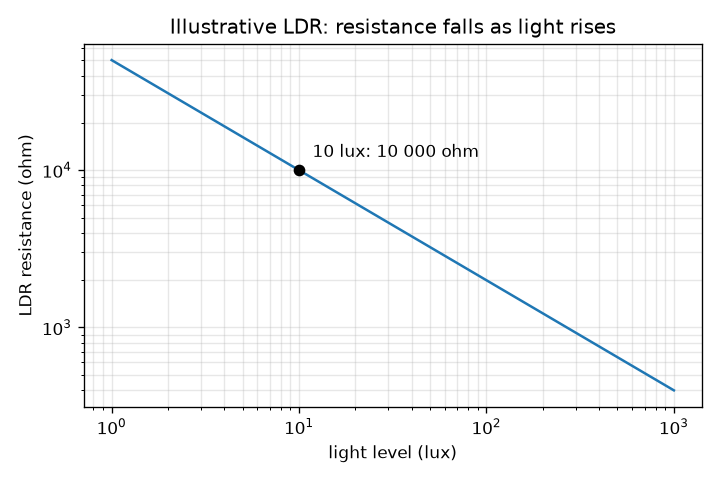
\includegraphics[width=0.85\linewidth]{figures/s01_ldr_curve.png}\\\small The illustrative LDR: a straight line on log-log axes, passing through (10 lux, 10 000 ohm).\end{center}

\subsection*{E. Worked example}
At 2 lux, what is the LDR resistance with the illustrative curve, and is the LED on with a 20 lux threshold?
\begin{enumerate}[nosep]
\item Light divided by 10: 2 / 10 = 0.2.
\item R = 10 000 * 0.2 \textasciicircum{} (-0.7). Since 0.2 \textasciicircum{} (-0.7) = 5 \textasciicircum{} 0.7 = 3.085, R = 10 000 * 3.085 = 30 852 ohm.
\item Compare with the threshold: 2 lux is below 20 lux, so the room is dark enough.
\item The comparator says 'dark', the transistor closes and the LED is ON.
\item Sanity check: 2 lux is darker than the 10 lux anchor, so the resistance must be above 10 000 ohm. It is.
\end{enumerate}
\textbf{Answer.} R is about 30 850 ohm and the LED is ON.

\subsection*{F. Questions}
\begin{enumerate}[nosep]
\item \textbf{Conceptual.} Why is a sensor whose resistance changes useful for a controller? Why do we also need a separate 'decision' block instead of connecting the LDR straight to the LED?
\item \textbf{Numerical.} Using R = 10 000 * (lux / 10) \textasciicircum{} (-0.7), find the LDR resistance at 1 lux and at 1 000 lux. By what factor do they differ? Sanity check the factor.
\item \textbf{Graph and simulation interpretation.} In the app's graph, the curve is steep on the left and nearly flat on the right. What does that say about how well an LDR distinguishes 5 lux from 15 lux compared with 405 lux from 415 lux?
\item \textbf{Design and optimisation challenge.} Design: a path light should turn on at dusk. Compare thresholds of 5 lux and 50 lux. Which would you choose and why? Give the LDR resistance at each threshold.
\end{enumerate}

\section{Session 2: The divider, the LED resistor and the transistor}

\subsection*{A. Real-world problem}
A comparator and a transistor cannot read an LDR's resistance directly: they need a voltage. And an LED must never be connected straight to a supply or it burns out. For a night light that comes on below 20 lux, which resistor goes with the LDR, how big is the LED resistor, and what stops the transistor from only half switching on? All values are for a low-voltage educational circuit at 5 V; 'typical' values come from typical small parts and must be checked against a real data sheet.

\subsection*{B. Concept and theory}
Put a fixed resistor R in series with the LDR across the supply Vcc. The voltage across R is V = Vcc R / (R + R\_ldr): small in the dark (R\_ldr large), large in the light. The comparator calls it dark when V falls below a threshold V\_th. At the threshold light level the divider gives exactly V\_th, so R\_ldr = R (Vcc - V\_th) / V\_th; with V\_th = Vcc / 2 the two resistors are equal, so R = R\_ldr(threshold). An LED has a nearly fixed forward voltage Vf (about 2 V for red, typical); its resistor takes the rest: R\_led = (Vcc - Vf) / I, with about 10 mA typical for an indicator LED. The comparator cannot carry 10 mA, so it drives the base of an NPN transistor: the LED path is in the collector. Real current gain is unreliable (it varies several times between parts), so for a switch we use a forced gain of about 10: I\_B = I\_C / 10 and R\_B = (V\_drive - V\_BE) / I\_B, with V\_BE about 0.7 V (typical). Too little base current leaves the transistor half on: the LED is dim and the transistor itself dissipates I\_C V\_CE. Resistors come in standard values (E12 series), so we pick the nearest suitable part.

\begin{itemize}[nosep]
\item Vcc: supply voltage (5) (V)
\item R: fixed resistor in the divider (ohm)
\item V: divider output voltage (V)
\item V\_th: comparator threshold voltage (V)
\item Vf: LED forward voltage (about 2, typical) (V)
\item I: LED current (about 10 mA, typical) (A)
\item V\_BE: base-emitter voltage (about 0.7, typical) (V)
\item I\_B, I\_C: base and collector currents (A)
\item R\_led, R\_B: LED resistor and base resistor (ohm)
\end{itemize}

\begin{equation*}
V=V_{cc}\,\frac{R}{R+R_{\mathrm{ldr}}}
\end{equation*}

\begin{equation*}
R=R_{\mathrm{ldr}}(\text{threshold})\,\frac{V_{th}}{V_{cc}-V_{th}}
\end{equation*}

\begin{equation*}
R_{\mathrm{led}}=\frac{V_{cc}-V_f}{I}
\end{equation*}

\begin{equation*}
I_B=\frac{I_C}{10},\qquad R_B=\frac{V_{\mathrm{drive}}-V_{BE}}{I_B}
\end{equation*}

\begin{center}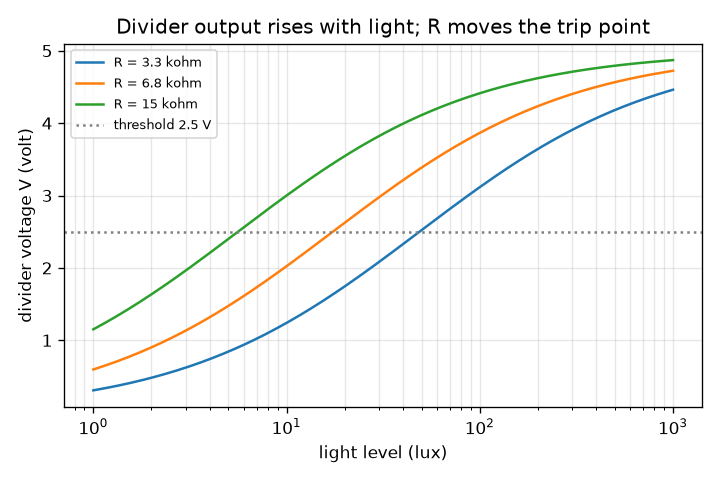
\includegraphics[width=0.85\linewidth]{figures/s02_divider_voltage.png}\\\small Divider voltage against light: a bigger fixed resistor trips at a lower light level.\end{center}

\subsection*{E. Worked example}
Design a night light for 5 V that turns on below 20 lux, using the illustrative LDR, a red LED at about 10 mA, an NPN transistor and V\_th = Vcc / 2. Find R, R\_led and R\_B, and say what threshold you really get.
\begin{enumerate}[nosep]
\item LDR at 20 lux: R\_ldr = 10 000 * (20 / 10) \textasciicircum{} (-0.7) = 10 000 * 0.6156 = 6 156 ohm.
\item With V\_th = 2.5 V = Vcc / 2, R = R\_ldr = 6 156 ohm. E12 neighbours: 5.6 kilo-ohm (trips at 22.9 lux) and 6.8 kilo-ohm (trips at 17.3 lux). Choose 6.8 kilo-ohm, or use a 10 kilo-ohm trimmer for an adjustable threshold.
\item LED resistor: (5 - 2) / 0.010 = 300 ohm, next E12 value up: 330 ohm, so I = 3 / 330 = 9.09 mA.
\item Base current for forced gain 10: I\_B = 9.09 / 10 = 0.909 mA. R\_B = (5 - 0.7) / 0.000909 = 4 730 ohm, E12 value at or below: 4.7 kilo-ohm, so I\_B = 0.915 mA.
\item Check: with V\_CE(sat) = 0.2 V the LED gets (5 - 2 - 0.2) / 330 = 8.48 mA, so the actual forced gain is 8.48 / 0.915 = 9.3, which is under 10. The transistor is saturated and dissipates about 8.48 mA * 0.2 V = 1.7 mW.
\end{enumerate}
\textbf{Answer.} R = 6.8 kilo-ohm (trips at 17.3 lux instead of exactly 20), R\_led = 330 ohm (9.09 mA), R\_B = 4.7 kilo-ohm (I\_B = 0.915 mA, LED current 8.5 mA).

\subsection*{F. Questions}
\begin{enumerate}[nosep]
\item \textbf{Conceptual.} Why do we size the base resistor for a forced gain of 10 when the transistor's gain might be 100 or more?
\item \textbf{Numerical.} A blue LED has Vf = 3.0 V (typical) and should carry 15 mA from 5 V. Find the LED resistor (pick an E12 value at or above the result) and the actual current, then the base resistor for forced gain 10 with a 5 V drive (E12 at or below).
\item \textbf{Graph and simulation interpretation.} In the divider graph the 15 kilo-ohm curve crosses 2.5 V at a lower light level than the 3.3 kilo-ohm curve. Read the two crossing light levels, and explain why a bigger R trips at a lower light level.
\item \textbf{Design and optimisation challenge.} Design an automatic night light that turns on below 30 lux with V\_th = 2.5 V: choose R from E12 and state the real trip level, choose R\_led and R\_B for a 10 mA red LED, and say how you would make the threshold adjustable.
\end{enumerate}

\section{Session 3: A controller you can trust: hysteresis, tolerances and logic}

\subsection*{A. Real-world problem}
At dusk the light does not fall smoothly: clouds, trees and passing cars make it wobble, so a comparator with one threshold flips the LED on and off, on and off, whenever the noisy light crosses it. That 'chatter' annoys people and wears relays. And every real part is a little different from its label. How do we make the controller decide once, and how far can we trust its trip point? A related question appears in safety design: how do you build an alarm that fires when either of two independent safety conditions is violated? This session is a low-voltage educational simulation, not a validated design tool.

\subsection*{B. Concept and theory}
A Schmitt trigger is a comparator with two thresholds: the LED turns on when the sensor voltage falls below V\_LO and turns off only when it rises above V\_HI; in between it keeps its state (memory). With our divider, V\_LO = 2.25 V and V\_HI = 2.75 V correspond to light levels found from lux = 10 (R10 / R\_ldr)\textasciicircum{}(1/gamma) with R\_ldr = R (Vcc - V) / V. The synthetic day follows log10(lux) = 1.3 + 3.2 sin(2 pi (t - 6) / 24) with t in hours, times a seeded random cloud factor exp(sigma n), where n is smoothed noise (AR(1), coefficient 0.8). Without clouds the switching times can be solved exactly, so the simulation is validated against them. A Monte Carlo run draws many circuits with random part values and looks at the spread of the trip point. For digital logic, signals are 0 or 1. The alarm for 'condition A or condition B is violated' is OR: its truth table is 0, 1, 1, 1. De Morgan's law says A OR B equals NOT(NOT A AND NOT B), so the same alarm can be built from NOT gates and a NAND. A gate simulator evaluates a list of gates in order, and a truth table is checked on all 2\textasciicircum{}n input rows (exhaustively).

\begin{itemize}[nosep]
\item V\_LO, V\_HI: Schmitt thresholds (2.25 and 2.75) (V)
\item sigma: cloud strength: standard deviation of ln(lux) noise (0.35) (no unit)
\item t: time of day (h)
\item switches: number of LED state changes in 24 h (count)
\item E: energy over the day (Wh)
\item A, B: the two alarm conditions (1 = violated) (no unit)
\end{itemize}

\begin{equation*}
\log_{10}(\text{lux})=1.3+3.2\sin\!\left(\frac{2\pi (t-6)}{24}\right)
\end{equation*}

\begin{equation*}
\text{lux}(V)=10\left(\frac{R_{10}}{R\,(V_{cc}-V)/V}\right)^{1/\gamma}
\end{equation*}

\begin{equation*}
t_{\text{fall}}=6+\frac{24}{2\pi}\left(\pi-\arcsin s\right),\quad t_{\text{rise}}=6+\frac{24}{2\pi}\arcsin s,\quad s=\frac{\log_{10}(\text{lux}_{th})-1.3}{3.2}
\end{equation*}

\begin{equation*}
A\ \mathrm{OR}\ B=\overline{\overline{A}\cdot\overline{B}}\quad\text{(De Morgan)}
\end{equation*}

\begin{center}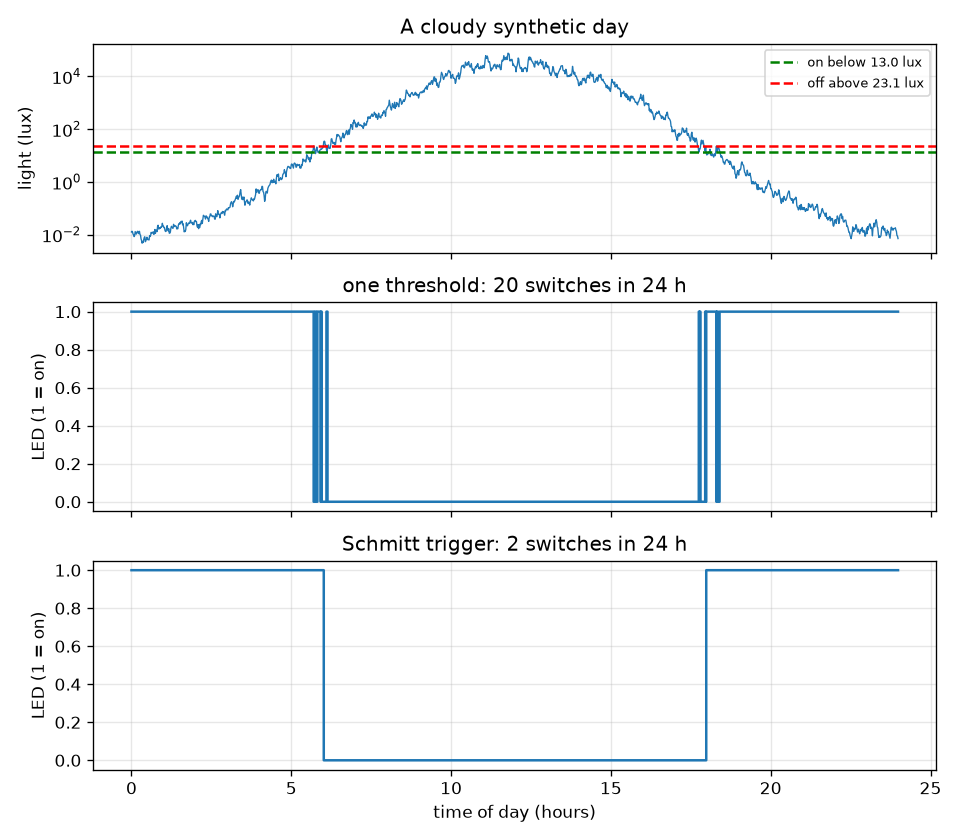
\includegraphics[width=0.85\linewidth]{figures/s03_day_simulation.png}\\\small A cloudy synthetic day: light with the two threshold levels, then the LED with one threshold (20 switches) and with the Schmitt trigger (2 switches).\end{center}

\subsection*{E. Worked example}
For the divider with R = 6.8 kilo-ohm and Schmitt thresholds V\_LO = 2.25 V and V\_HI = 2.75 V, find the two light levels by hand, then the evening switch-on time and the LED on-hours of a day without clouds, and compare with the simulation.
\begin{enumerate}[nosep]
\item At 2.25 V: R\_ldr = 6 800 * (5 - 2.25) / 2.25 = 8 311 ohm, so lux = 10 * (10 000 / 8 311) \textasciicircum{} (1 / 0.7) = 13.0 lux. The LED turns on below 13.0 lux.
\item At 2.75 V: R\_ldr = 6 800 * (5 - 2.75) / 2.75 = 5 564 ohm, so lux = 10 * (10 000 / 5 564) \textasciicircum{} (1.4286) = 23.1 lux. The LED turns off above 23.1 lux.
\item Evening switch-on: s = (log10(13.0) - 1.3) / 3.2 = -0.058, arcsin s = -0.058 rad, so t = 6 + (24 / 2 pi)(pi + 0.058) = 18.22 h (about 18:13).
\item Morning switch-off: s = (log10(23.1) - 1.3) / 3.2 = 0.0199, t = 6 + (24 / 2 pi)(0.0199) = 6.08 h (about 06:05).
\item On-hours = (24 - 18.22) + 6.08 = 11.86 h; the simulation (1 minute steps) gives 11.85 h. They agree to within one time step. With a cloudy day (seed 7) the single threshold switches 20 times and the Schmitt trigger 2 times.
\end{enumerate}
\textbf{Answer.} The LED switches on below 13.0 lux and off above 23.1 lux; on a clean day it comes on at 18.22 h, goes off at 6.08 h and is on 11.85 h (simulation) against 11.86 h (hand calculation).

\subsection*{F. Questions}
\begin{enumerate}[nosep]
\item \textbf{Conceptual.} Why does hysteresis stop chatter without smoothing the light signal? And why is XOR the wrong gate for an alarm that must fire when either of two conditions is violated?
\item \textbf{Numerical.} A wider Schmitt band uses V\_LO = 2.0 V and V\_HI = 3.0 V with R = 6.8 kilo-ohm. Find the light levels for on and off. Compare the ratio of off-level to on-level with that of the 2.25 V and 2.75 V pair.
\item \textbf{Graph and simulation interpretation.} In the day-simulation figure, why do all the extra switches of the single-threshold comparator cluster near dawn and dusk and none occur at noon or midnight?
\item \textbf{Design and optimisation challenge.} Design: a machine has two independent safety conditions, A (temperature too high) and B (pressure too high). The alarm must fire when either is violated. Write the truth table, choose the gate, and say how you would make a broken sensor wire fail safe. Then add a manual-override input for a maintenance person who may silence the alarm.
\end{enumerate}

\section{Real-world mini-project}
\textbf{Add a manual override to the night light.} The night light must obey two buttons: FORCE\_ON (hold the light on, even in daylight) and FORCE\_OFF (hold it off, even at night). If both are pressed, off wins. Use the gate simulator in Session 3 (the \texttt{OVERRIDE} netlist) and \texttt{simulate\_day} with the seed 7 day. Test a day where FORCE\_ON is held from 12:00 to 13:00 and FORCE\_OFF from 22:00 to 23:30. Then answer a power question: the whole day may use at most 0.65 Wh; with FORCE\_OFF unchanged and FORCE\_ON starting at 12:00, what is the longest whole-hour FORCE\_ON window that fits?

\section{The path ahead}
\begin{enumerate}[nosep]
\item \textbf{Session 4: Debounce instead of hysteresis.} A controller with a single threshold plus a debounce timer, compared with the Schmitt trigger.
\item \textbf{Session 5: Fade the LED in and out.} A brightness output between 0 and 1 that follows the decision gradually.
\item \textbf{Session 6: Make the trip point immune to the supply.} A comparator reference that follows the supply or a stable fixed reference with a regulated supply, checked by Monte Carlo.
\item \textbf{Session 7: Calibrate the LDR from measurements.} A fit from six noisy readings of resistance against light, then a controller built from the fitted curve.
\item \textbf{Session 8: A latching alarm with reset.} A gate-level alarm with inputs A, B and RESET whose output stays on after the cause is gone.
\end{enumerate}

\section{Answers and hints}

\subsection*{Session 1}
\begin{enumerate}[nosep]
\item \textbf{Conceptual.} Hint: A resistance is not yet a yes/no answer, and the LED needs a definite on or off. Solution: A change of resistance can be turned into a voltage that follows the light (Session 2), which a circuit can measure. But the LED needs a clear on/off command at a chosen light level: the comparator turns the continuous signal into yes or no, and the transistor then supplies the LED current. Without the decision block the LED would just glow a little brighter or dimmer, and a small sensor signal could not carry the LED current.
\item \textbf{Numerical.} Hint: 1 lux gives lux/10 = 0.1 and 1 000 lux gives 100. Solution: At 1 lux: 10 000 * 0.1 \textasciicircum{} (-0.7) = 10 000 * 5.012 = 50 119 ohm. At 1 000 lux: 10 000 * 100 \textasciicircum{} (-0.7) = 10 000 * 0.03981 = 398 ohm. Factor = 50 119 / 398 = 125.9, which equals 1 000 \textasciicircum{} 0.7 = 125.9 (a thousand times more light, resistance about 126 times less). Units: ohm.
\item \textbf{Graph and simulation interpretation.} Hint: Compare the change of resistance for the same change of light at the two places. Solution: On the left (dim light) a small change of light changes the resistance a lot, so dim light levels are easy to tell apart. On the right a change of 10 lux changes the resistance by only a few ohm, so bright light levels are hard to tell apart. That is why LDR controllers work best around dusk (tens of lux) and not for measuring bright daylight accurately.
\item \textbf{Design and optimisation challenge.} Hint: Think about when each threshold is reached, energy use and safety, and compute R at both. Solution: R at 5 lux = 16 245 ohm; R at 50 lux = 3 241 ohm. A 50 lux threshold switches on earlier, in deep twilight, which is safer for walkers but uses more LED hours; 5 lux switches on when it is really dark, saving energy but leaving a dim period. A sensible compromise for a path is about 20 to 30 lux. Trade-off: safety and comfort against energy, and later (Session 3) against chatter near the threshold.
\end{enumerate}

\subsection*{Session 2}
\begin{enumerate}[nosep]
\item \textbf{Conceptual.} Hint: Datasheet gain is a range, and gain falls with temperature and when the transistor is hard on. Solution: The gain varies a lot between parts and with temperature and current. If we counted on gain 100 and a part has gain 40, the transistor would not carry the full LED current: it would be only half on, so the LED would be dim and the transistor would heat. Feeding 10 times more base current than the gain 100 would need makes the switch fully on for every realistic part, at the cost of a little extra base current.
\item \textbf{Numerical.} Hint: R\_led = (5 - 3) / 0.015, and use the actual LED current to size I\_B. Solution: R\_led = 2 / 0.015 = 133 ohm, E12 value up = 150 ohm, actual current = 2 / 150 = 13.3 mA. I\_B = 1.33 mA, R\_B = 4.3 / 0.00133 = 3 225 ohm, E12 value down = 2.7 kilo-ohm, giving I\_B = 1.59 mA. Sanity check: I\_B = 1.59 mA is a little more than one tenth of 13.3 mA, so the forced gain is under 10 and the transistor is safely saturated.
\item \textbf{Graph and simulation interpretation.} Hint: Use R = R\_ldr at 2.5 V and the LDR curve: where is R\_ldr = 15 000 ohm and where is it 3 300 ohm? Solution: R = R\_ldr at the trip, so 15 000 ohm gives lux = 10 * (10 000 / 15 000)\textasciicircum{}(1/0.7) = 5.6 lux and 3 300 ohm gives 48.7 lux. A bigger fixed resistor needs a bigger LDR resistance to balance it, and the LDR is only that large when it is darker. So bigger R means a darker trip point.
\item \textbf{Design and optimisation challenge.} Hint: R\_ldr at 30 lux with the curve, then E12 nearest; the LED and base values are as in the worked example. Solution: R\_ldr(30 lux) = 10 000 * 3 \textasciicircum{} (-0.7) = 4 635 ohm. The nearest E12 value is 4.7 kilo-ohm, which trips at 29.4 lux (very close). R\_led = 330 ohm (9.09 mA) and R\_B = 4.7 kilo-ohm as before. For an adjustable threshold replace R by a 10 kilo-ohm trimmer in series with a small fixed resistor: at 10 kilo-ohm it trips at 10.0 lux, and 3.3 kilo-ohm trips at 48.7 lux, so the range covers 10 to 49 lux. Assumptions: illustrative LDR curve, typical LED and transistor values; a real build needs a data sheet check and a test.
\end{enumerate}

\subsection*{Session 3}
\begin{enumerate}[nosep]
\item \textbf{Conceptual.} Hint: Think of the gap between the two thresholds, and what XOR does when both inputs are 1. Solution: With two thresholds the signal must travel the whole gap (here 2.75 - 2.25 = 0.5 V) to undo a decision, and a cloud-sized wobble is smaller than the gap, so the state does not flip back. The signal is not smoothed: it still wobbles, but the decision has memory. XOR is 1 only when exactly one input is 1, so when both conditions are violated at once (the worst case) the alarm would stay silent. OR is 1 whenever at least one input is 1.
\item \textbf{Numerical.} Hint: Use R\_ldr = R (Vcc - V) / V and lux = 10 (R10 / R\_ldr) \textasciicircum{} (1 / 0.7) for each voltage. Solution: At 2.0 V: R\_ldr = 6 800 * 3 / 2 = 10 200 ohm, lux = 10 * (10 000 / 10 200) \textasciicircum{} 1.4286 = 9.7 lux. At 3.0 V: R\_ldr = 6 800 * 2 / 3 = 4 533 ohm, lux = 31.0 lux. Ratio of levels: 31.0 / 9.7 = 3.2 (against 23.1 / 13.0 = 1.8 for the narrower band), so the wider band tolerates larger cloud swings but turns the light on later and off later by more.
\item \textbf{Graph and simulation interpretation.} Hint: Where is the light close to the threshold level, and how big is the noise compared with the distance? Solution: A switch needs the noisy light to cross the threshold. At noon the light is thousands of lux, far above the 17 lux threshold, and at midnight it is a small fraction of a lux, far below it, so noise (a factor of about 1.4) cannot bridge the gap. Only around dusk and dawn, when the clean light passes through the threshold, does the noise push the signal back and forth across it. In the seed 7 day the comparator switched 20 times and the Schmitt trigger twice.
\item \textbf{Design and optimisation challenge.} Hint: Four rows for two inputs; think about what a broken wire reads, and whether silencing should be allowed to hide a dangerous state. Solution: Truth table (A, B -\textgreater{} alarm): 0 0 -\textgreater{} 0; 0 1 -\textgreater{} 1; 1 0 -\textgreater{} 1; 1 1 -\textgreater{} 1, which is OR. It can also be built as NAND(NOT A, NOT B). Fail-safe: if a sensor wire breaks it usually reads 'no signal' (0). With 1 = violated that would look safe, so use active-low sensing (0 = violated, 1 = healthy): a broken wire then reads violated and raises the alarm. Override: alarm\_out = alarm AND NOT silence is only acceptable for a limited time, with a visible indicator, and never for a safety condition that endangers people; in a real system this logic is certified. Trade-off: more inputs and checks give more safety but also more false alarms. This is a teaching exercise only.
\end{enumerate}

\section{How to join}
Read \texttt{CONTRIBUTING.md} in the repository, then pick an issue labelled \texttt{good first issue}. Repository: \url{https://github.com/KrunalPanchal1995/openledcontrol}

\end{document}
